% = = = = = = = = = = = = = = = = = = = = = %
%                    Bios                   %
% = = = = = = = = = = = = = = = = = = = = = %

\chapter{Bios}

\section{Li Shi}

\begin{minipage}{0.25\textwidth}
  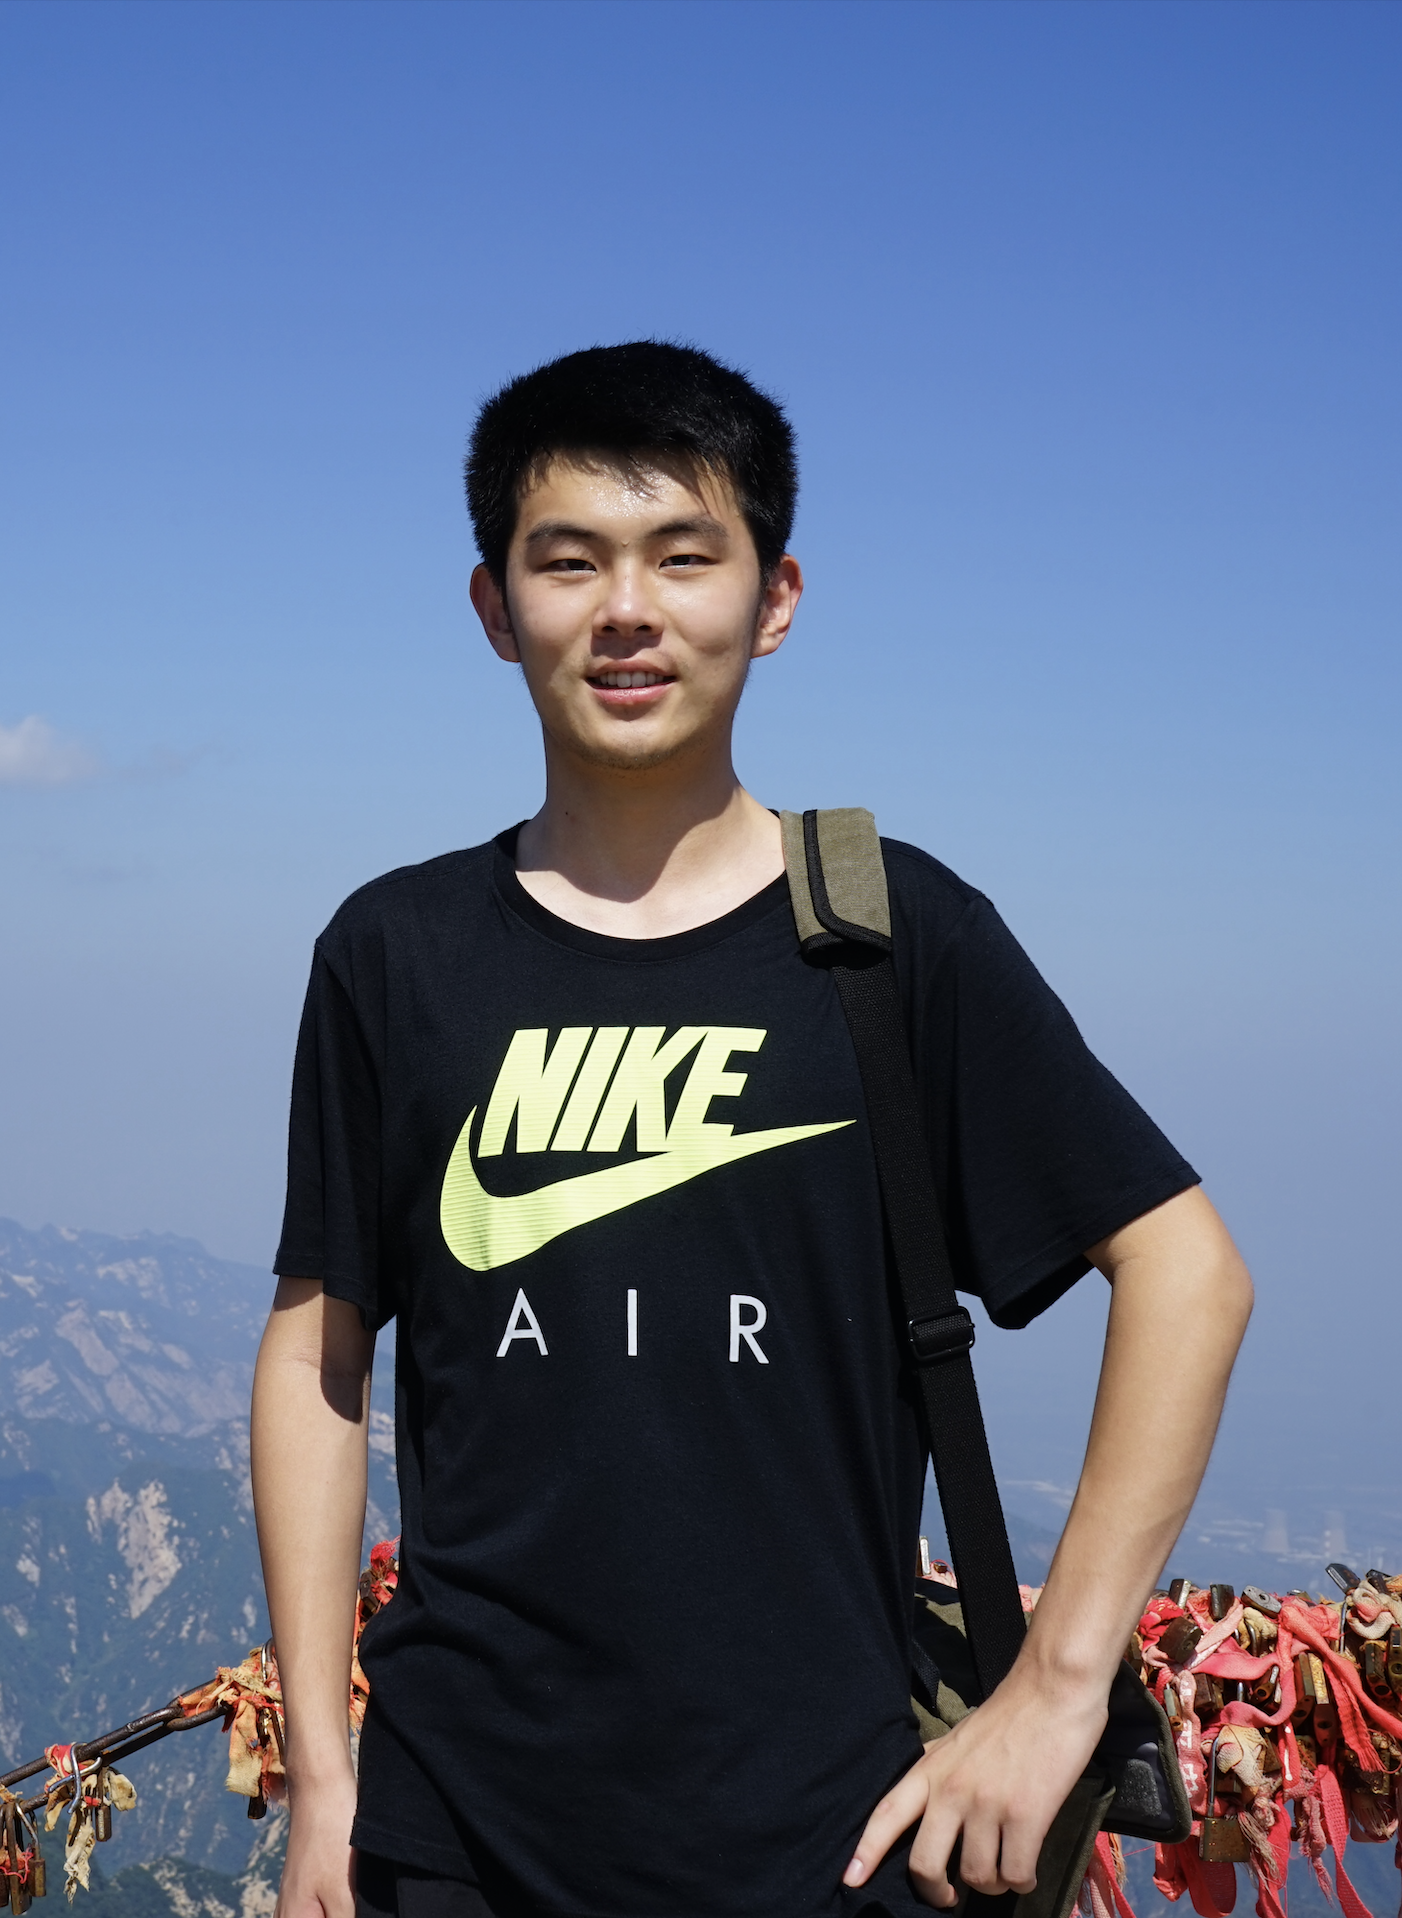
\includegraphics[width=1.2in,height=1.5in,clip,keepaspectratio]{figure/sl.png}
\end{minipage}
\begin{minipage}{0.75\textwidth}\raggedright
  \begin{tabular}{l l}
    \textbf{Major}          & Electrical \& Computer Engineering \\
    \textbf{Student ID}     & 517370910032 \\
    \textbf{SJTU Email}     & \url{shili2017@sjtu.edu.cn} \\
    \textbf{Personal Email} & \url{shili2048@gmail.com} \\
    \textbf{Phone}          & +86-14782059981
  \end{tabular}
\end{minipage}

I am Li Shi, a senior undergraduate major in ECE at JI. I like studying photography, watching sci-fi movies, eating Chinese food (especially Sichuan cuisine), and sleeping. Also, I enjoy playing with kittens and puppies.

Before the capstone design project, I have been working on the High-Level Synthesis project instructed by Prof. Weikang Qian at JI for about 2 years, during which I accumulated some experience on digital design, software engineering, compiler design, etc. Meanwhile, I once worked as an intern at Apple, where I participated in developing a CPU simulator and studied computer architecture by myself. My interests include digital design, embedded systems, computer architecture, etc. In 2022, I will start my journey in M.S. in ECE program at Carnegie Mellon University.


\section{Zhiyuan Liu}

\begin{minipage}{0.25\textwidth}
  \includegraphics[width=1.2in,height=1.5in,clip,keepaspectratio]{figure/lzy.png}
\end{minipage}
\begin{minipage}{0.75\textwidth}\raggedright
  \begin{tabular}{l l}
    \textbf{Major}          & Electrical \& Computer Engineering \\
    \textbf{Student ID}     & 517370910240 \\
    \textbf{SJTU Email}     & \url{angelinaliu@sjtu.edu.cn} \\
    \textbf{Personal Email} & \url{?} \\
    \textbf{Phone}          & +86-?
  \end{tabular}
\end{minipage}

My name is Zhiyuan Liu, a senior student in JI major in ECE. I like drawing, photography, playing video games, and basketball. Besides, I like to assemble computers by myself. Before the capstone design project, I studied VE270 Introduction to Logic Design and VE370 Intro to Computer Organization in JI, and I also learned VE470 Computer Architecture by myself. I am very interested in computer architecture. I once worked as an intern at Microsoft and I participated in feature development for products there.

This fall, I will become a regular employee of Microsoft.


\section{Yiqiu Sun}

\begin{minipage}{0.25\textwidth}
  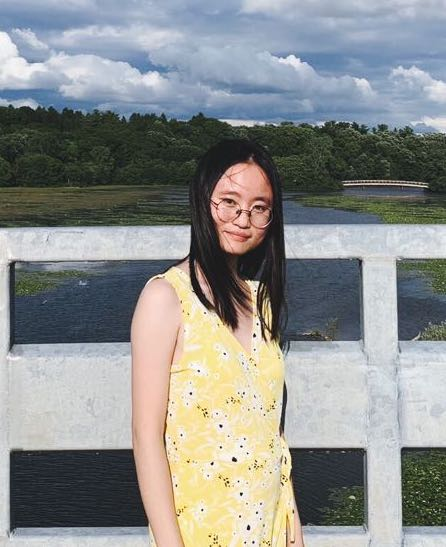
\includegraphics[width=1.2in,height=1.5in,clip,keepaspectratio]{figure/syq.jpeg}
\end{minipage}
\begin{minipage}{0.75\textwidth}\raggedright
  \begin{tabular}{l l}
    \textbf{Major}          & Electrical \& Computer Engineering \\
    \textbf{Student ID}     & 517370910020 \\
    \textbf{SJTU Email}     & \url{susansun@sjtu.edu.cn} \\
    \textbf{Personal Email} & \url{?} \\
    \textbf{Phone}          & +86-?
  \end{tabular}
\end{minipage}

My name is Yiqiu Sun. I major in ECE at JI and CE at University of Michigan. Interested in Computer Architecture and new computing techniques like approximate computing, I worked with Prof. John Hayes on stochastic computing and with Prof. Trevor Mudge on re-configurable accelerators. Meanwhile, my course experience of EECS 470 Computer Architecture at Michigan would help me better contribute to this project. This fall, I will pursue my Ph.D. degree in computer science in University of Illinois at Urbana-Champaign. With a research focus on In-Memory Computing, I would like to figure out a better communication scheme between processor and memory in the future.

Besides academics, I am interested in cooking and hiking. I also adopted two cats. They are Gomez and Kent. These two fluffy creatures are my best life companions.


\section{Jian Shi}

\begin{minipage}{0.25\textwidth}
  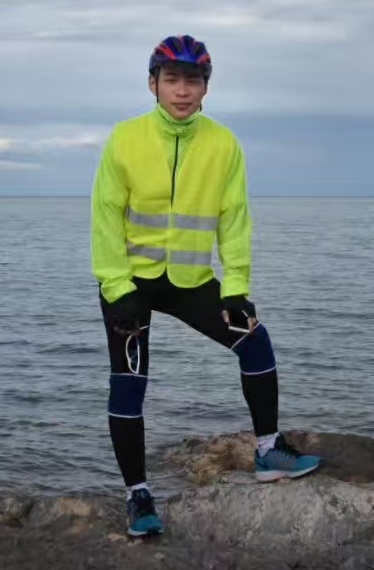
\includegraphics[width=1.2in,height=1.5in,clip,keepaspectratio]{figure/sj.jpg}
\end{minipage}
\begin{minipage}{0.75\textwidth}\raggedright
  \begin{tabular}{l l}
    \textbf{Major}          & Electrical \& Computer Engineering \\
    \textbf{Student ID}     & 517370910255 \\
    \textbf{SJTU Email}     & \url{timeshi@sjtu.edu.cn} \\
    \textbf{Personal Email} & \url{?} \\
    \textbf{Phone}          & +86-?
  \end{tabular}
\end{minipage}

I am Jian Shi, a senior student major in ECE at JI. I like taking photos, analyzing video games and swimming. Also, I am a full stack developer. I build and maintain an online server by myself. Starting from choosing hardware components in the server, to the deamon service written by myself, I learn a lot from this experience. Currently, the server has become my computing center. Whenever I have a task that can be processed or maintained by computer or network, I will write a program and throw it to my server. By the way, the test platform for this project is also based on my server.

This fall, I will continue my Ph.D. degree at JI under Prof. Weikang Qian's guidance. I think this project will help a lot in my future Ph.D. study.


\section{Yichao Yuan}

\begin{minipage}{0.25\textwidth}
  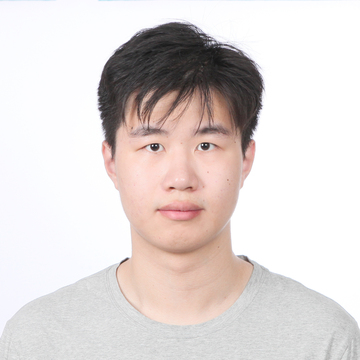
\includegraphics[width=1.2in,height=1.5in,clip,keepaspectratio]{figure/yyc.jpg}
\end{minipage}
\begin{minipage}{0.75\textwidth}\raggedright
  \begin{tabular}{l l}
    \textbf{Major}          & Electrical \& Computer Engineering \\
    \textbf{Student ID}     & 517370910233 \\
    \textbf{SJTU Email}     & \url{yyc19990826@sjtu.edu.cn} \\
    \textbf{Personal Email} & \url{?} \\
    \textbf{Phone}          & +86-?
  \end{tabular}
\end{minipage}

My name is Yichao Yuan. I am a senior student in JI major in ECE. I like movies, graphics and various technology topics. I enjoy writing software and building hardware and the beauty of their interaction always amazes me. Before the capstone project, I have solid knowledge at each abstraction layer of hardware. In JI, VE270 and VE370 introduce basics about logic design and computer organization. In 2020 spring, I took CS152 and EECS151 in UC, Berkeley, which gave me advanced knowledge in computing architecture and digital design.

This fall, I will be an ECE M.S. student at University of Michigan, Ann Arbor.
